\section{Theory}
\subsection{Set up}
Let $\mathcal{V} \subset \mathbb{R}^m$, for some dimension $m \in \mathbb{N}$, be a finite set corresponding to the domain which represents the pixels/voxels at which we observe imaging data. Let $\mathcal{X} = \lbrace g: \mathcal{V} \rightarrow \mathbb{R}\rbrace$ be the set of real functions on $\mathcal{V}$ and let $\mathcal{Y} = \lbrace g: \mathcal{V} \rightarrow \lbrace 0,1 \rbrace \rbrace$ be the set of all functions taking the values 0 or 1. Suppose that we observe a calibration dataset $(X_i, Y_i)_{i = 1}^n$ of random images, where $X_i: \mathcal{V} \rightarrow \mathbb{R}$ represents the $i$th observed calibration image and $Y_i:\mathcal{V} \rightarrow \lbrace 0, 1\rbrace$ outputs labels at each $v \in \mathcal{V}$ giving 1s at the true location of the objects in the image $X_i$ that we wish to identify and 0s elsewhere. Let $\mathcal{P}(\mathcal{V})$ be the set of all subsets of $\mathcal{V}$.

Let $s:\mathcal{X} \times \mathcal{V} \rightarrow \mathbb{R}$ be a score function - trained on an independent dataset - such that given an image pair $(X,Y) \in \mathcal{X}\times \mathcal{Y}$, $s(X, v)$ is intended to be higher at the $v \in \mathcal{V}$ for which $Y(v) = 1$. The score function can for instance be the logit scores obtained from a deep neural network image segmentation method e.g. CITE. 
%Let $T(Y) = \left\lbrace v\in \mathcal{V}: Y(v) = 1 \right\rbrace$ correspond to the true location of the objects in the image $X$. 

In what follows we will use the calibration dataset to construct a confidence functions $I,O:  \mathcal{X}  \rightarrow \mathcal{P}(\mathcal{V})$ such that for a new image pair $(X,Y) \sim \mathcal{D}$, given error rates $\alpha_1, \alpha_2 \in (0,1)$ we have
\begin{equation}\label{eq:probstat1}
	\mathbb{P}\left( I(X) \subseteq \lbrace v\in \mathcal{V}: Y(v) = 1 \rbrace  \right) \geq 1 - \alpha_1, 
\end{equation}
\begin{equation}\label{eq:probstat2}
	\text{ and } 	\mathbb{P}\left( \lbrace v\in \mathcal{V}: Y(v) = 1 \rbrace \subseteq O(X)  \right) \geq 1 - \alpha_2.
\end{equation}
Here $I(X)$ and $O(X)$ serve as inner and outer confidence sets for the location of the true segmented mask. Their interpretation is that, up to the guarantees provided by the probabilistic statements \eqref{eq:probstat1} and \eqref{eq:probstat2}, we can be sure that for each $v\in I(X)$, $Y(v) = 1$ or that for each $v \not\in O(X)$, $Y(v) = 0$. See Figure \ref{fig:polpys} for an example of this in practice. Joint control over the events can also be guaranteed, either by sensible choices of $\alpha_1$ and $\alpha_2$ or by using the joint distribution of the maxima of the logit scores - see Section \ref{SS:joint}. 

In order to establish conformal confidence results we shall require the following exchangeablity assumption. 
\begin{assumption}\label{ass:ex}
		Given a new random image pair, $(X_{n+1},Y_{n+1})$, suppose that $(X_i, Y_i)_{i = 1}^{n+1}$ is an exchangeable sequence of random image pairs in the sense that 
	\begin{equation*}
		\left\lbrace (X_1,Y_1), \dots, (X_{n+1}, Y_{n+1}) \right\rbrace =_d \left\lbrace (X_{\sigma(1)}, Y_{\sigma(1)}), \dots, (X_{\sigma(n+1)}, Y_{\sigma(n+1)}) \right\rbrace
	\end{equation*}
	for any permutation $\sigma \in S_{n+1}$. Here $=_d$ denotes equality in distribution and $S_{n+1} $ is the group of permutations of the integers $\lbrace1, \dots, n+1\rbrace$.
\end{assumption}
Exchangeability or a variant is a standard assumption in the conformal inference literature \citep{Angelopoulos2021} and factilates coverage guarantees. It holds for instance if we assume that the collection $(X_i, Y_i)_{i = 1}^{n+1}$ is an i.i.d. sequence of image pairs but is more general and in principle allows for other dependence structures. 

\subsection{Marginal confidence sets}
In order to construct conformal confidence sets let $f_O, f_I:\mathbb{R} \rightarrow \mathbb{R}$ be increasing functions and for each $1\leq i \leq n$, let $\tau_i = \max_{v \in \mathcal{V}: Y_i(v) = 0} f_O(s(X_i,v))$ and $\gamma_i = \max_{v \in \mathcal{V}: Y_i(v) = 1} f_I(-s(X_i,v))$  be the maxima of the function transformed scores over the areas at which the true labels equal 0 and 1 respectively. Then we construct confidence sets as follows.
\begin{theorem}\label{thm:inner}
	(Marginal inner set)
	Under Assumption \ref{ass:ex}, given $\alpha_1 \in (0,1)$, let 
	\begin{equation*}
		\lambda_I(\alpha_1) = \inf\left\lbrace \lambda: \frac{1}{n} \sum_{i = 1}^n 1\left[ \gamma_i\leq \lambda \right] \geq \alpha_1 \right\rbrace.
	\end{equation*}
	be the upper $\alpha$ quantile of $(\gamma_i)_{i = 1}^n$and define $I(X) = \lbrace v \in \mathcal{V}: f_I(-s(X,v)) >\lambda_I(\alpha_2)  \rbrace $. Then,
	\begin{equation}\label{eq:probstat}
		\mathbb{P}\left( I(X) \subseteq\lbrace v\in \mathcal{V}: Y_{n+1} = 1 \rbrace \right) \geq 1 - \alpha_1.
	\end{equation}
\end{theorem}
\begin{proof}
	Let $\tau_{n+1}= \max_{v \in \mathcal{V}: Y_{n+1}(v) = 0} f_O(s(X_{n+1},v))$, Then exchangeability of the image pairs implies exchangeability of the sequence $(\tau_i)_{i = 1}^{n+1}$. In particular, as $\lambda_I(\alpha_1)$ is the $\alpha_1$ quantile of the distribution of $(\tau_i)_{i = 1}^{n}$, by Lemma 1 of \cite{} it follows that 
	\begin{equation*}
	\mathbb{P}\left(\gamma_{n+1} \leq \lambda_I(\alpha_1) \right) \geq 1 - \alpha_1. 
	\end{equation*}
	Now consider the event that $\gamma_{n+1}\leq \lambda_{\alpha}$, on this event, $ f_O(s(X_{n+1},v)) \leq \lambda_\alpha $
	for all $v \in \mathcal{V}$ such that $Y_{n+1}(v) = 0$. As such, given $u \in \mathcal{V}$ such that $ f_O(s(X_{n+1},u)) > \lambda_\alpha$, we must have $Y_{n+1}(u) = 1$ so it follows that $	\lbrace v\in \mathcal{V}: Y(v) = 1 \rbrace \subseteq O(X) $ and in particular that 
	\begin{equation*}
	\mathbb{P}\left( \lbrace v\in \mathcal{V}: Y(v) = 1 \rbrace \subseteq O(X)  \right) \geq \mathbb{P}\left(\gamma_{n+1} \leq \lambda_I(\alpha_1) \right) \geq 1 - \alpha_1. 
\end{equation*}
\end{proof}
\noindent Similarly for the outer set we have
\begin{theorem}\label{thm:outer}
	(Marginal outer set)
	Under Assumption \ref{ass:ex}, given $\alpha_2 \in (0,1)$, let 
	\begin{equation*}
		\lambda_O({\alpha_2})= \inf\left\lbrace \lambda: \frac{1}{n} \sum_{i = 1}^n 1\left[ \tau_i\leq \lambda \right] \geq \alpha_2 \right\rbrace.
	\end{equation*}
	be the upper $\alpha$ quantile of $(\gamma_i)_{i = 1}^n$and define $O(X) = \lbrace v \in \mathcal{V}: f_O(s(X,v)) >\lambda_O(\alpha_2)  \rbrace $. Then,
	\begin{equation}\label{eq:probstat}
		\mathbb{P}\left( \lbrace v\in \mathcal{V}: Y_{n+1}(v) = 1 \rbrace \subseteq O(X_{n+1}) \right) \geq 1 - \alpha_2.
	\end{equation}
\end{theorem}
\noindent The proof of Theorem \ref{thm:outer} follows that of Theorem \ref{thm:inner} and is thus omitted. 

%\begin{remark}
%	Importantly the coverage of the sets $U_M(X)$ and $V_M(X)$ is not jointly valid and so when using these results the choice of inner versus outer set must be made in advance.
%\end{remark}

%\subsection{Confidence sets for connected components}

%\subsection{Full conformal confidence sets}
%We have so far assumed that we have a calibration dataset available, separate from the training data used to contruct the score function, on which we can learn cutoffs and use them to provide conformal confidence sets, using split conformal prediction. As an alternative, we could instead use full conformal prediction in which the entire dataset is used to both train the model and to provide conformal uncertainty. 
%
%To do so let $s_{}$
%
%\begin{remark}
%	Full conformal confidence sets come with the same drawbacks as full conformal inference. In particular they can be very computationally expensive to generate because they require retraining the model for each XXX. As a result, this approach does not scale well when the dataset is large and will often not be practical.
%\end{remark}

\subsection{Joint confidence sets}\label{SS:joint}
Instead of focussing on marginal control one can instead spend all of the $\alpha$ available to construct sets which have a joint probabilistic guarantees. This gain comes at the expense of a loss of precision. The simplest means of constructing jointly valid confidence sets is via the marginal sets themselves.
\begin{corollary}\label{cor:weighting}
	(Joint from marginal) Assume Assumption \ref{ass:ex} holds and given $\alpha \in (0,1)$ and $\alpha_1, \alpha_2 \in (0,1)$ such that $\alpha_1 + \alpha_2 \leq \alpha$, define $I(X)$ and  $O(X)$ as in Theorems \ref{thm:inner} and \ref{thm:outer}. Then 
	\begin{equation}
		\mathbb{P}\left( I(X) \subseteq \lbrace v\in \mathcal{V}: Y_{n+1}(v) = 1 \rbrace \subseteq O(X)  \right) \geq 1 - \alpha. 
	\end{equation}
\end{corollary}
Alternatively joint control can be obtained using the joint distribution of the maxima of the logit scores as follows.
\begin{theorem}\label{thm:joint}
	(Joint coverage) Assume that Assumption \ref{ass:ex} holds. Given $\alpha \in (0,1)$, let 
	\begin{equation*}
		\lambda(\alpha) = \inf\left\lbrace \lambda: \frac{1}{n} \sum_{i = 1}^n 1\left[ \max(\tau_i, \gamma_i) \leq \lambda \right] \geq \alpha \right\rbrace
	\end{equation*}
	to be the upper $\alpha$-quantile of the distribution of $\max(\tau_i, \gamma_i)$ over $1 \leq i \leq n$. Let $O(X) = \lbrace v \in \mathcal{V}: f_O(s(X,v)) >  \lambda(\alpha) \rbrace $ and $I(X) = \lbrace v \in \mathcal{V}: f_I(-s(X,v)) >	\lambda(\alpha) \rbrace $. Then,
\begin{equation}\label{eq:probstat}
	\mathbb{P}\left( I(X) \subseteq \lbrace v\in \mathcal{V}: Y(v) = 1 \rbrace \subseteq O(X) \right) \geq 1 - \alpha.
\end{equation}
\end{theorem}
\begin{proof}
	Exchangeability of the image pairs implies exchangeability of the sequence $(\tau_i)_{i = 1}^{n+1}$. Moreover on the event that $\max(\tau_{n+1}, \gamma_{n+1}) \leq \lambda_{\alpha}$. In particular $\tau_{n+1} \leq \lambda_\alpha$ and $\gamma_{n+1} \leq \lambda_\alpha$ on this event so the result following via a proof similar to that of Theorem \ref{thm:inner}.
\end{proof}

\begin{remark}
	The advantage of Corollary \ref{cor:weighting} is that the resulting inner and outer sets provide pivotal inference - not favouring one side or the other - which can be important when the distribution of the score function is asymmetric. Moreover the levels $\alpha_1$ and $\alpha_2$ can be used to provide a greater weight to either inner or outer sets whilst maintaining joint coverage. Theorem \ref{thm:joint} may instead be useful when there are strong levels of dependence between $\tau_1$ and $\gamma_1$. In practice this dependence is often low and scale differences in the scores can lead to a severe lack of pivotality. As such in practice it may be better to construct joint sets using Corollary \ref{cor:weighting}. 
\end{remark}

%Typically in our applications, $X_{n+1}$ will observed with $Y$ unknown.
%
%%%%
% $c: \mathcal{X} \times \mathcal{V} \rightarrow \mathbb{R} $ such that given  and letting $I(X) = \lbrace v \in \mathcal{V}: c(X,v) = 1\rbrace$, we have
%\begin{equation*}
%	\mathbb{P}\left( Y(v) = 1 \text{ for all } v \in I(X) \right) \geq 1 - \alpha.
%\end{equation*}
%This corresponds to controlling  $\mathbb{P}\left( Y(v) = 0 \text{ for all } v \in I(X) \right) $, i.e. the probabilty of making an error, to a level $\alpha.$ This error rate is analogous to the familywise error rate from the multiple testing setting, an observation that allows us to control it using the distribution of the maximum in the spirit of Westphal-Young. 
%
%To do so, let $T_i = \max_{v \in \mathcal{V}: Y_i(v) = 0} s(X_i,v)$ and define
%\begin{equation*}
%	\lambda_{\alpha} = \inf\left\lbrace \lambda: \frac{1}{n} \sum_{i = 1}^n 1\left[ T_i \leq \lambda \right] \geq \alpha \right\rbrace.
%\end{equation*}
%be the upper $\alpha$-quantile of the distribution of the maximum of the score function of the observed image over the areas at which the true label is equal to 0. Then define the classifier, $c: \mathcal{X} \times \mathcal{V}$ such that
%\begin{equation*}
%	c(X, v) = 1[s(X,v)> \lambda_{\alpha}].
%\end{equation*}
%\begin{theorem}
%	Given $(X,Y) \sim \mathcal{D}$ independent of $(X_i, Y_i)_{i = 1}^n$, we have
%	\begin{equation*}
%		\mathbb{P}\left( Y(v) = 1 \text{ for all } v \in I(X) \right) \geq 1 - \alpha.
%	\end{equation*}
%\end{theorem}
%\begin{proof}
%	Suppose that $Y(v) = 0$ for some $v \in I(X)$, then it follows that $s(X,v) > \lambda_\alpha$ and conversely. Thus the event $\lbrace Y(v) = 0 \text{ for some } v \in I(X) \rbrace$ occurs if and only if $\max_{v \in \mathcal{V}: Y(v) = 0} s(X,v) >  \lambda_\alpha$. Let $T_{n+1} = \max_{v \in \mathcal{V}: Y(v) = 0} s(X,v)$. Then the vector $(T_1, \dots, T_{n+1})$ is exchangeable, so arguing as in XXX, it follows that $T_{n+1}$ is equally to lie between (or before/after) the values $T_1, \dots, T_n$. As such 
%	$\mathbb{P}\left( T_{n+1} > \lambda_{\alpha}\right) \leq \alpha$
%	and the result follows.
%\end{proof}

\subsection{Better segmentors provide more precise conformal confidence sets}
Given two real random variables, $A$ and $B$ write $ A \succeq B$ to indicate that $\mathbb{P}\left( A > t \right) \geq \mathbb{P}\left( B > t \right)$ for all $t \in \mathbb{R}$. Then we have the following result. 
\begin{theorem}
	Suppose that $(X_i, Y_i)_{i = 1}^{n+1}$ is an i.i.d. sequence, and let $s, t: \mathcal{V} \rightarrow \mathbb{R}$ be two score functions. Assume that 
	$\max_{v \in \mathcal{V}: Y_1(v) = 0} s_v(X_{1}) \succeq \max_{v \in \mathcal{V}: Y_1(v) = 0} s_v(X_{1}) $
\end{theorem}

\subsection{Optimizing score transformations on  a learning dataset}
%\subsubsection{Setting aside a learning dataset}
The choice of score transformations $f_I$ and $f_O$ is extremely important and can have a large impact on the size of the conformal confidence sets. The best choice depends on both the distribution of the data and on the nature of the output of the trained segmentor used to calculate the scores. We thus recommend setting aside a learning dataset independent from both the calibration dataset, used to compute the conformal thresholds, and the test dataset. 

In order to make efficient use of the data available, the learning dataset can in fact contain some or all of the data used to train the image segmentor. This data is assumed to be independent of the calibration and test data and so can be used to learn the best score transformations without compromising validity . The advantage of doing so is that less additional data needs to be set aside or collected for the purposes of learning a score function. Moreover it allows for additional data to be used to train the model resulting in better segmentation performance. The disadvantage is that machine learning models typically overfit their training data meaning that certain score functions may appear to perform better on this data than they do in practice. The choice of whether to include training data in the learning dataset thus depends on the quantity of data available and the quality of the segmentation model.
%\subsubsection{Useful score transformations}

\section{Application to Polpys tumor segmentation}
In order to illustrate and validate our approach we consider the problem of polpys tumor segmentation from XXX images. To do so we use the same dataset as in XXX and XXX in which 1782 poplys images, with available ground truth masks were combined from 5 open-source datasets (published in \cite{KVASIR2017}, \cite{Hyperkvasir2020} \cite{Bernal2012}, \cite{Silva2014}). As in XXX, logit scores were obtained using the PraNet model \cite{PraNet2020}, which is based on the Unet architecture CITE CHECK! 

\subsection{Choosing a score transformation}
In order to optimize the size of our confidence sets we set aside 282 of the 1782 polpys images to form a learning dataset with which to choose the best score transformation. Note that since the learning dataset is independent of the remaining 1500 images set-aside, we can study it as much as we like without compromising the validity of the follow-up analysis in Section \ref{SS:val}. 

The score transformations we considered were the identity (after softmax transformation), distance transformations of the predicted masks and smoothing using a Gaussian kernel. Given a score function $s$ and a threshold $t \in \mathbb{R}$ let $B(t)$ be the set of points on the boundary of the set $\lbrace v \in \mathcal{V}: s(v) > t$ obtained by applying the marching squares algorithm CITE. Distance transformation scores are then obtained as following


The PraNet scores for several typical examples are shown, after applying these transformations, in Figure XXX.  From these we see that PraNet assigns a high softmax score to the polpys regions which decreases in the regions directly around the  boundary of the tumor before returning to a higher level away from the polpys. This results in tight inner sets but large outer sets as the model struggles to identify where the tumor ends. 

Further examples are shown in Appendix XXX. 

Based on the images set aside for alpha weighting we decided to use $\alpha_1 = 0.02$ and $\alpha_2 = 0.08$ to ensure a joint coverage of $90\%$. This ratio was chosen in light of the fact that in this data identifying where a given tumor ends appears to be more challenging than identifying pixels where we are sure that there is a tumor. For comparison we also present the results of an equal weighting scheme.


\begin{figure}
		\centering
		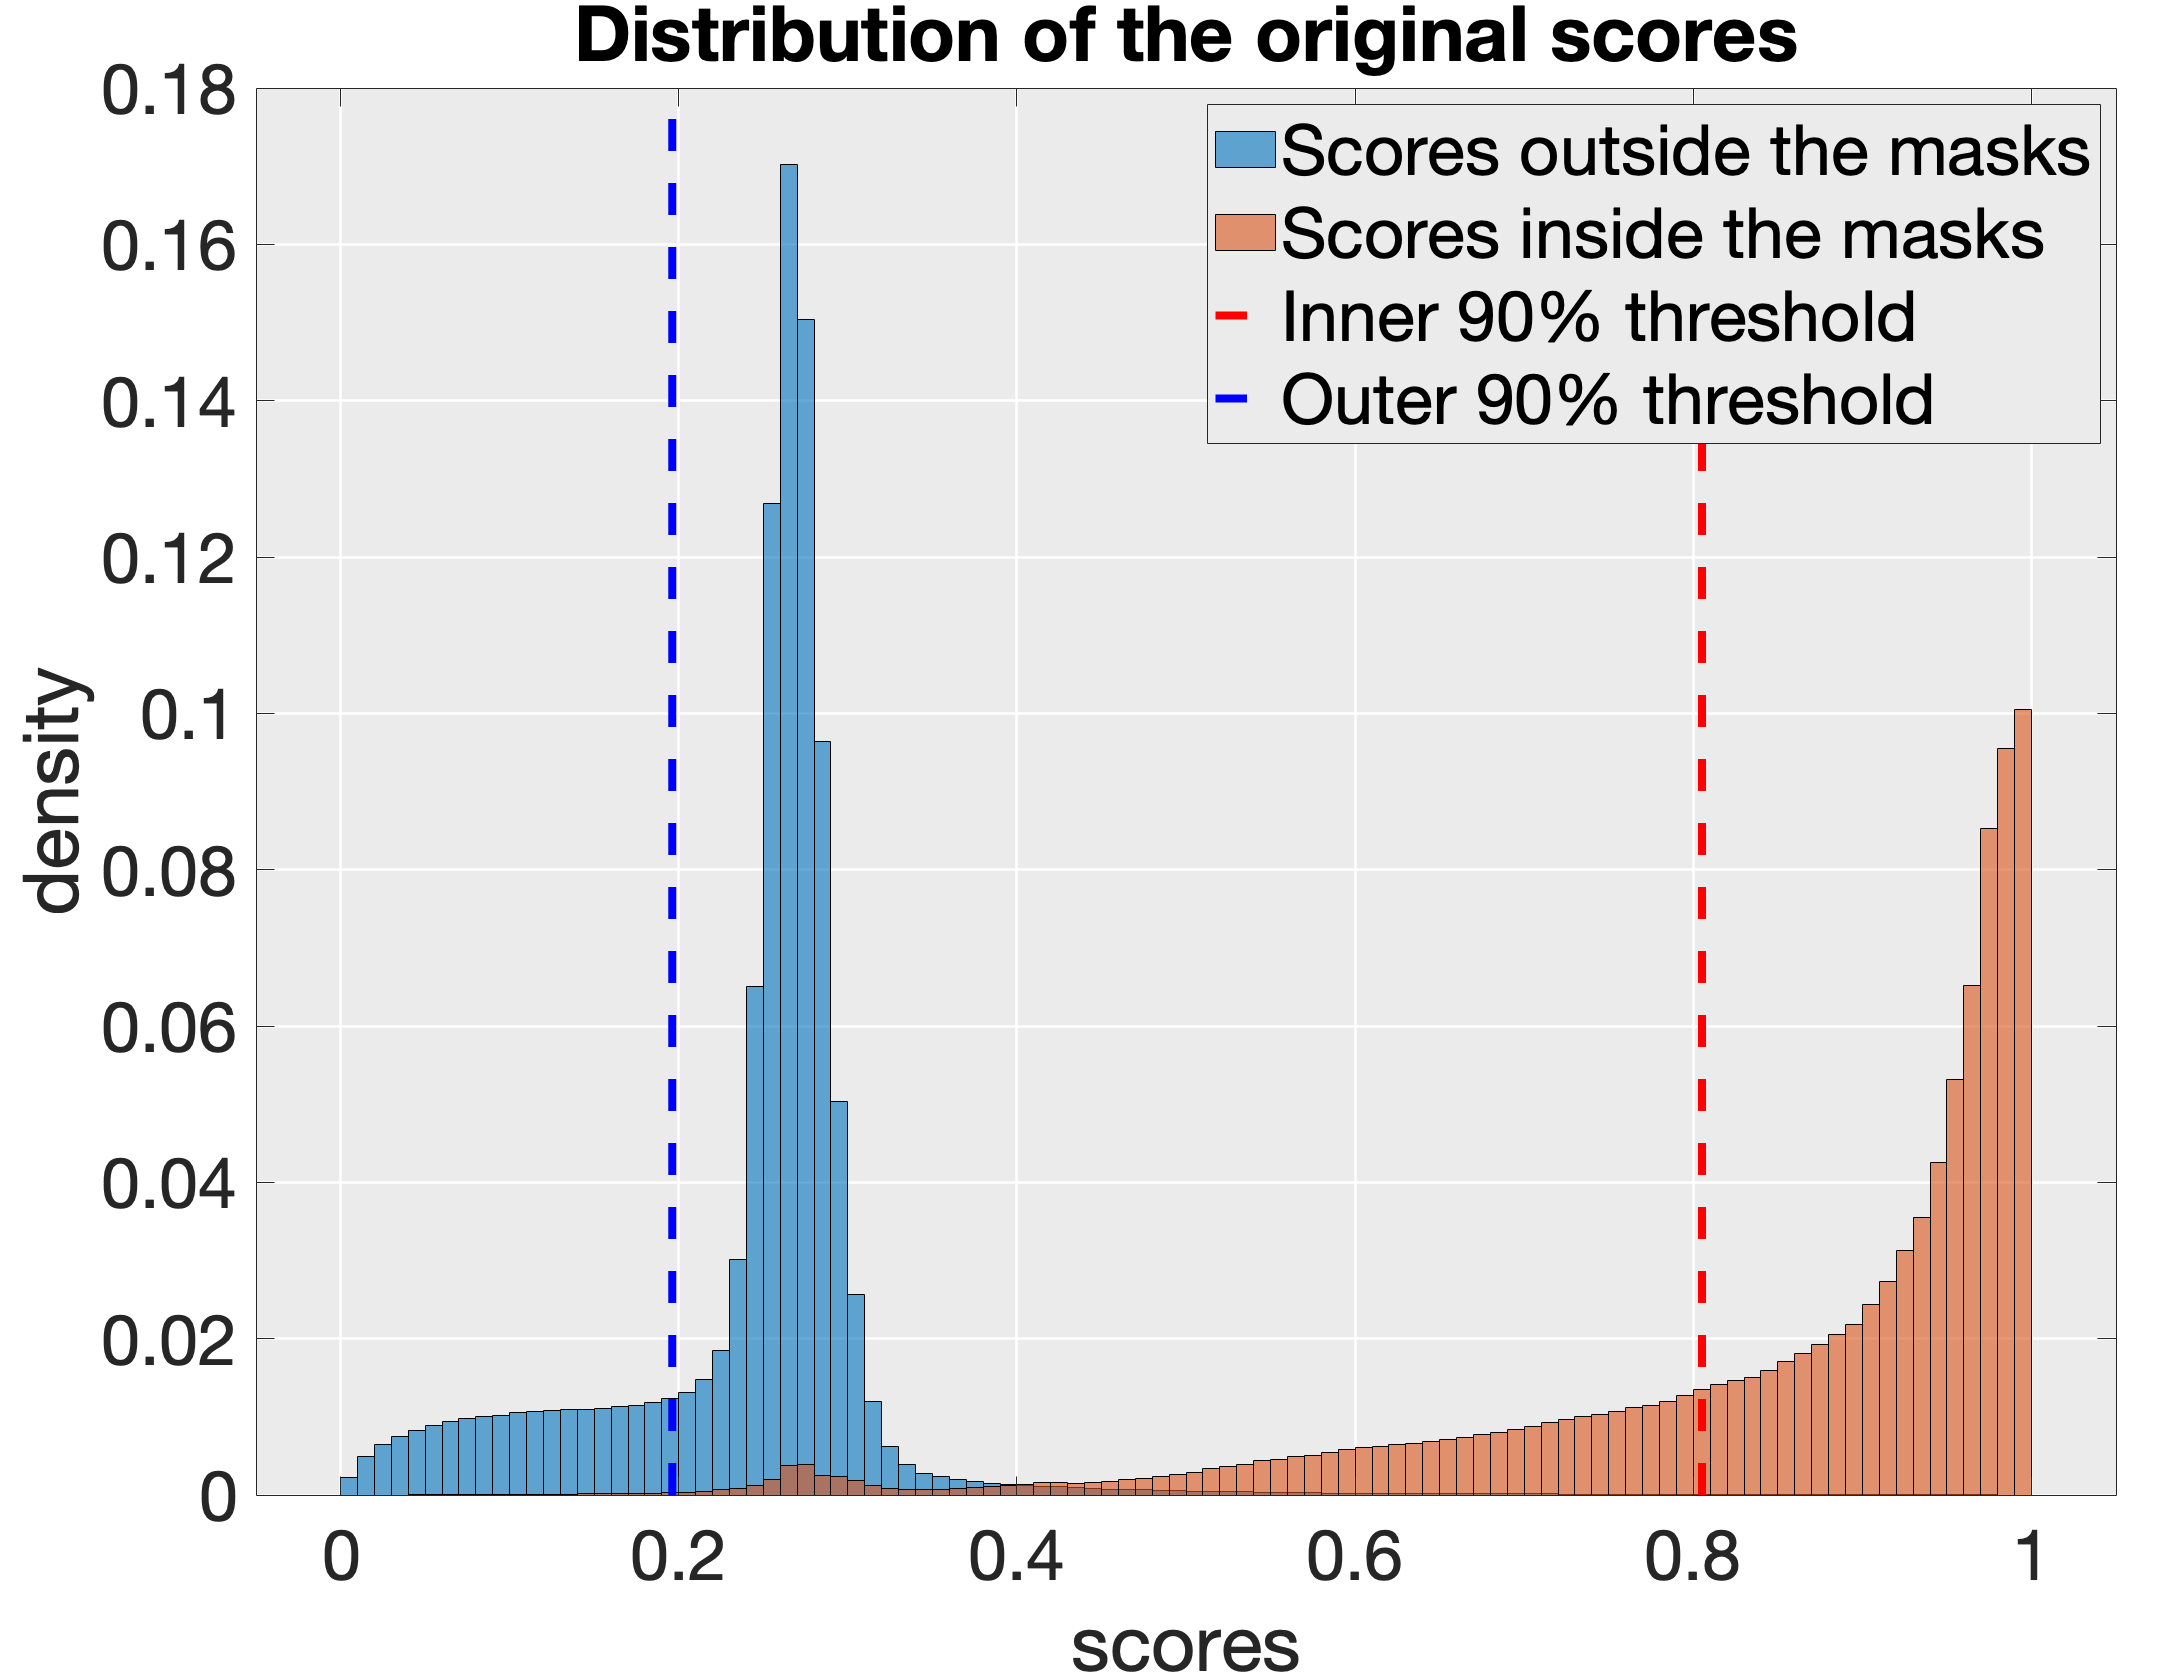
\includegraphics[width=0.3\textwidth]{../figures/learning/origscores.png}
		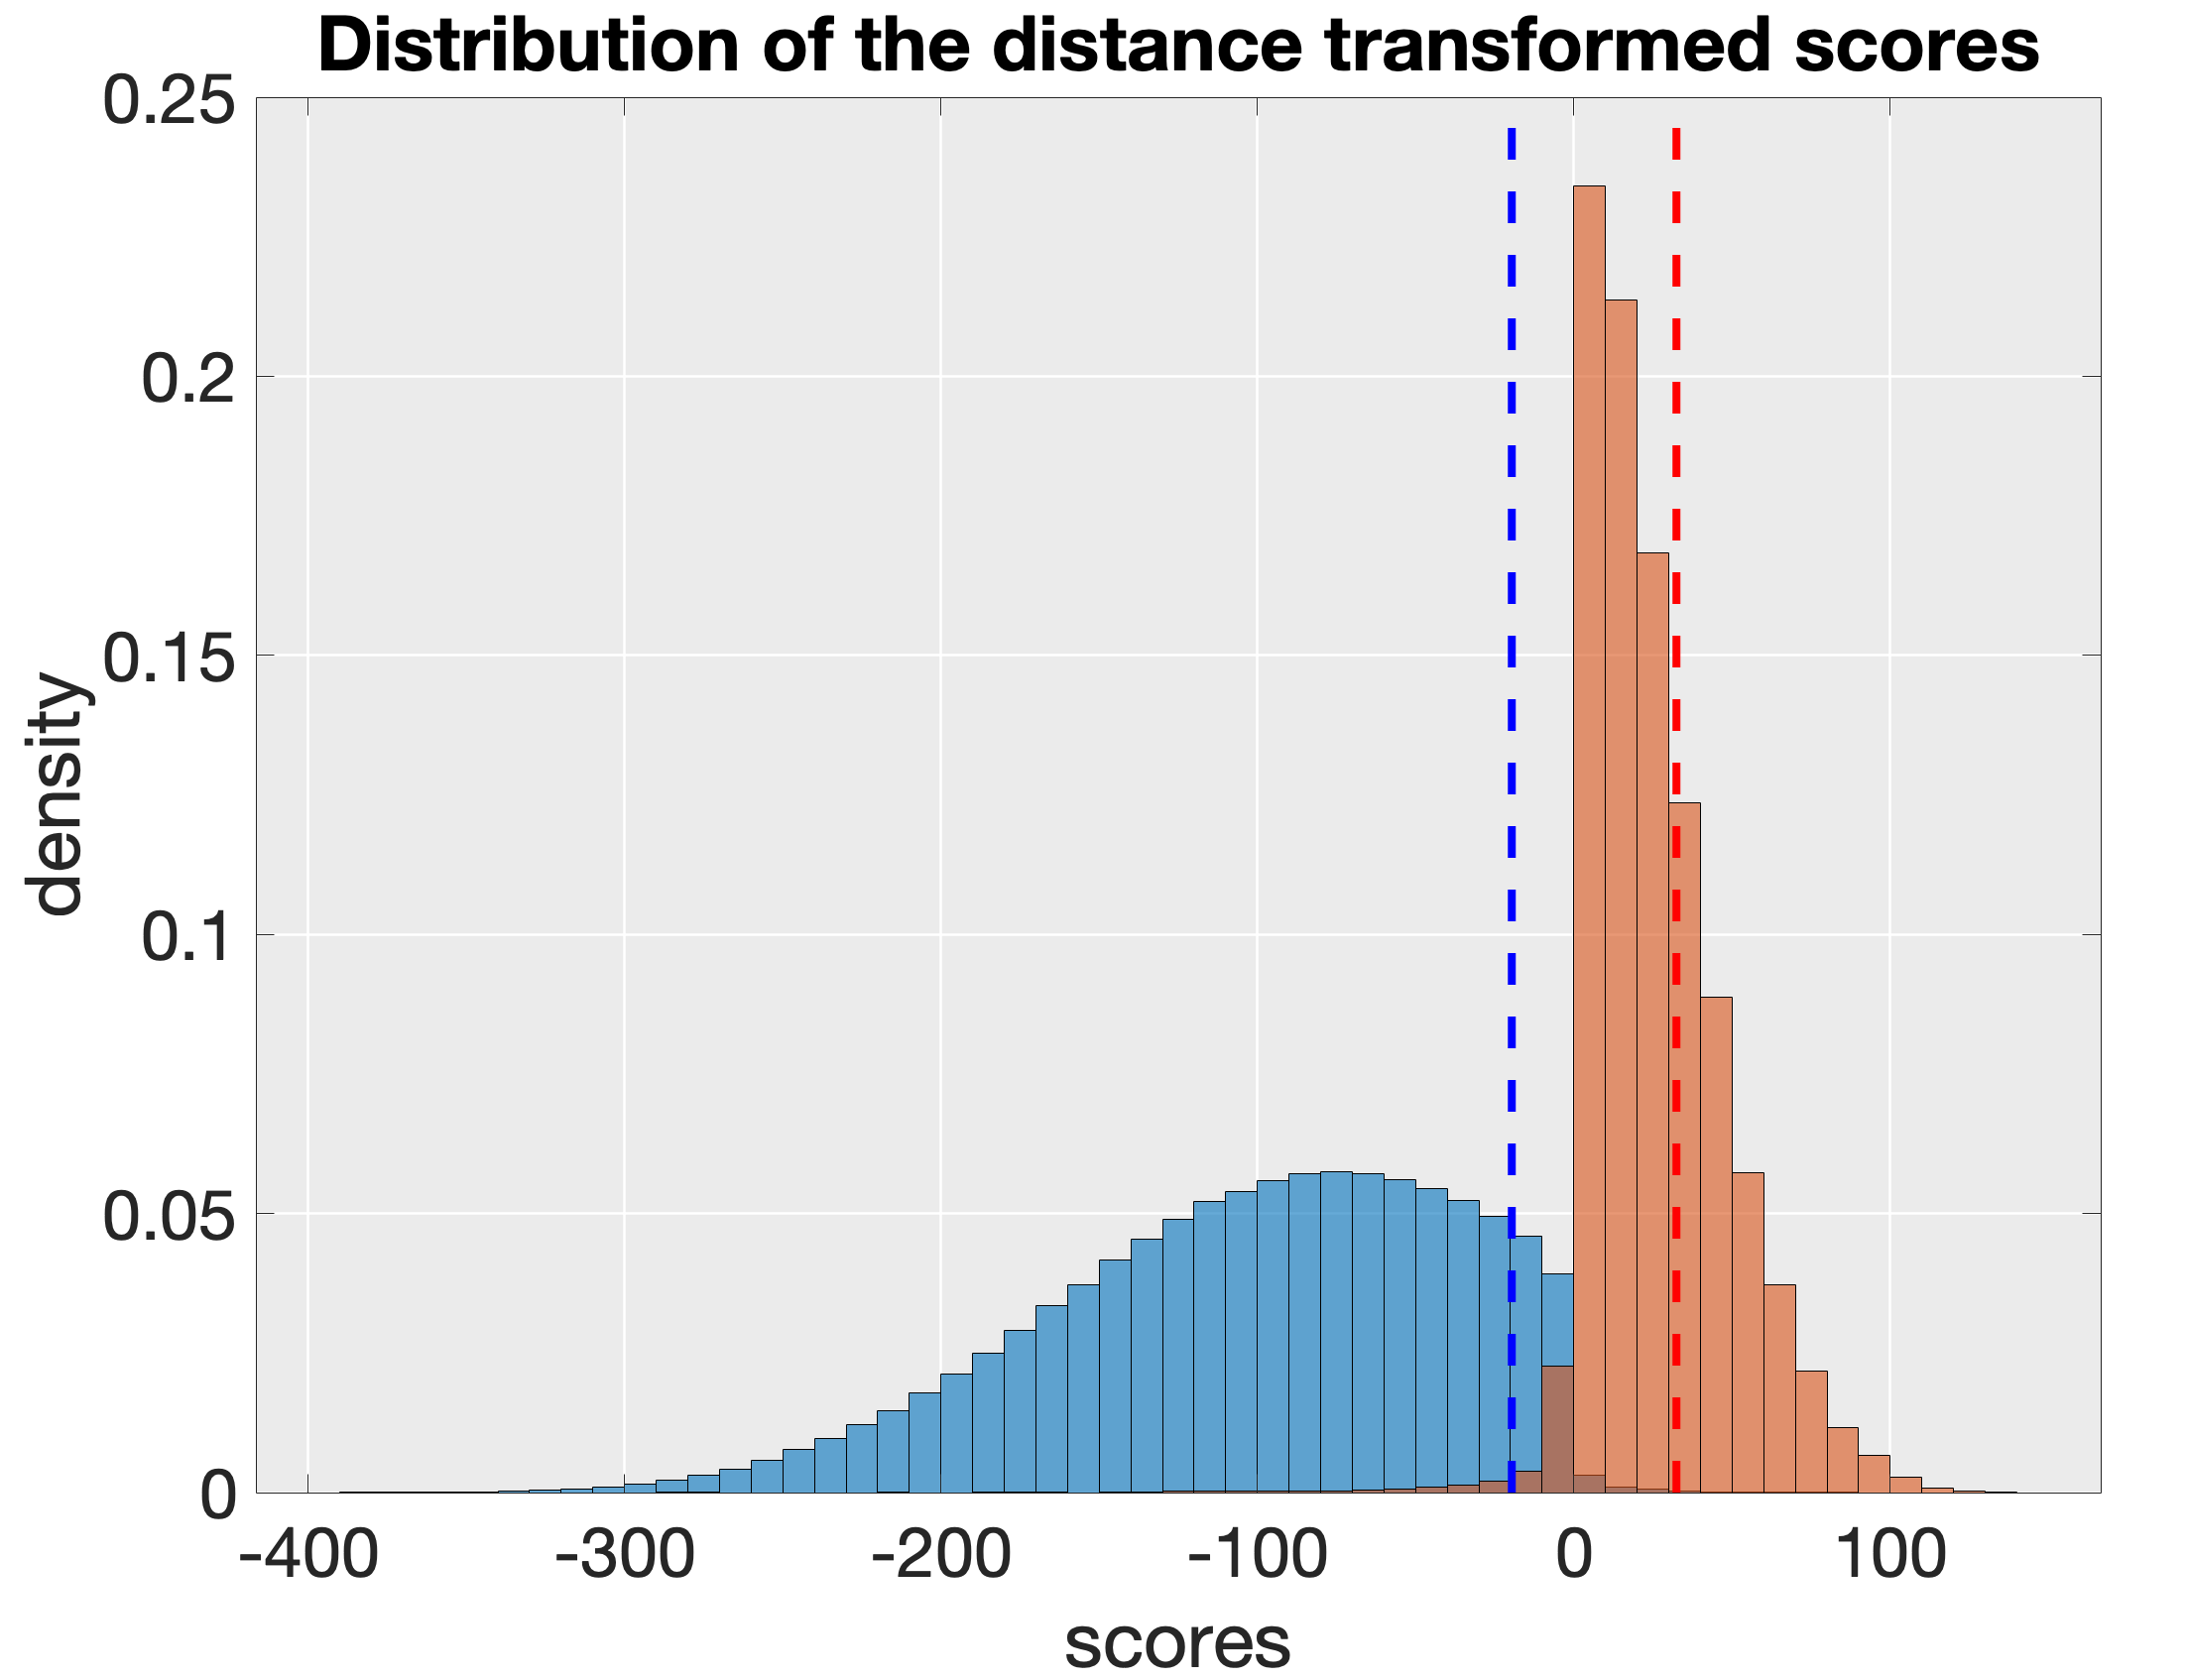
\includegraphics[width=0.3\textwidth]{../figures/learning/distscores.png}
		\label{scorehists}
\end{figure}
From the histograms in Figure \ref{scorehists} we can see that thresholding the scores at the inner threshold captures most of the data. However this is not the case for the outer threshold. From Figure XXX we can see that confidence sets based on the original scores struggle to identify where the tumor ends, resulting in very large sets. 

\begin{figure}
	\centering
	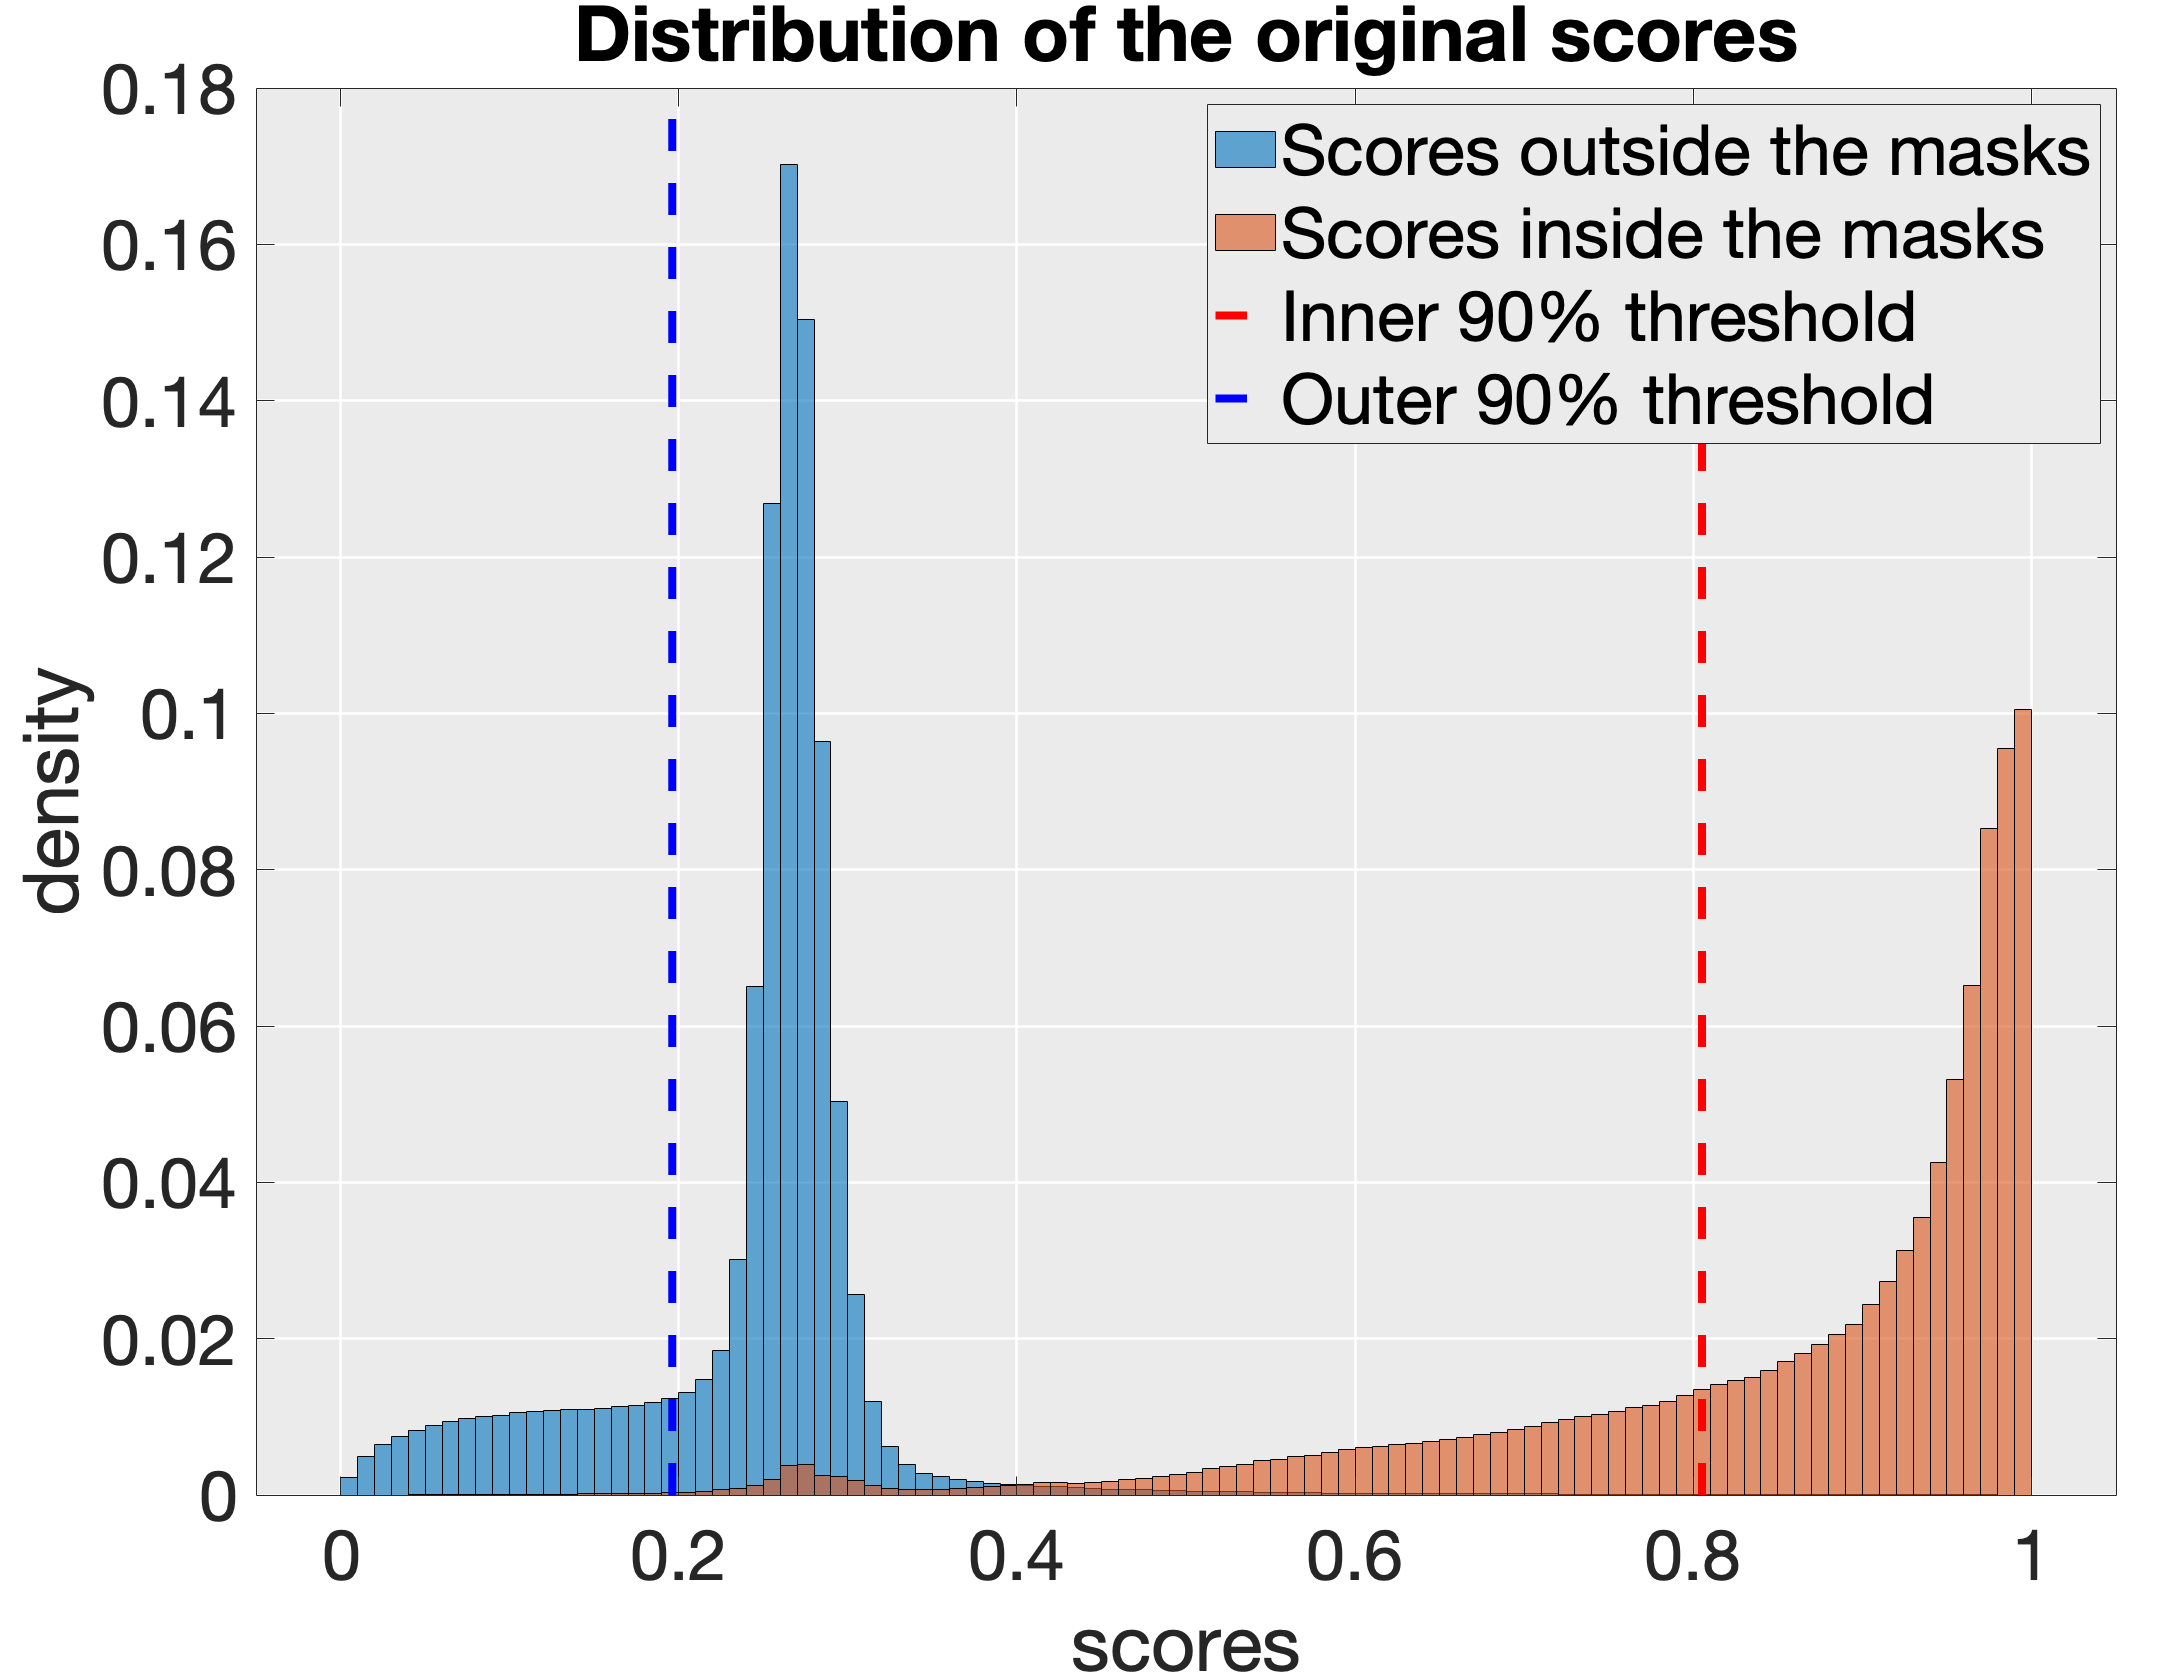
\includegraphics[width=0.3\textwidth]{../figures/learning/origscores.png}
	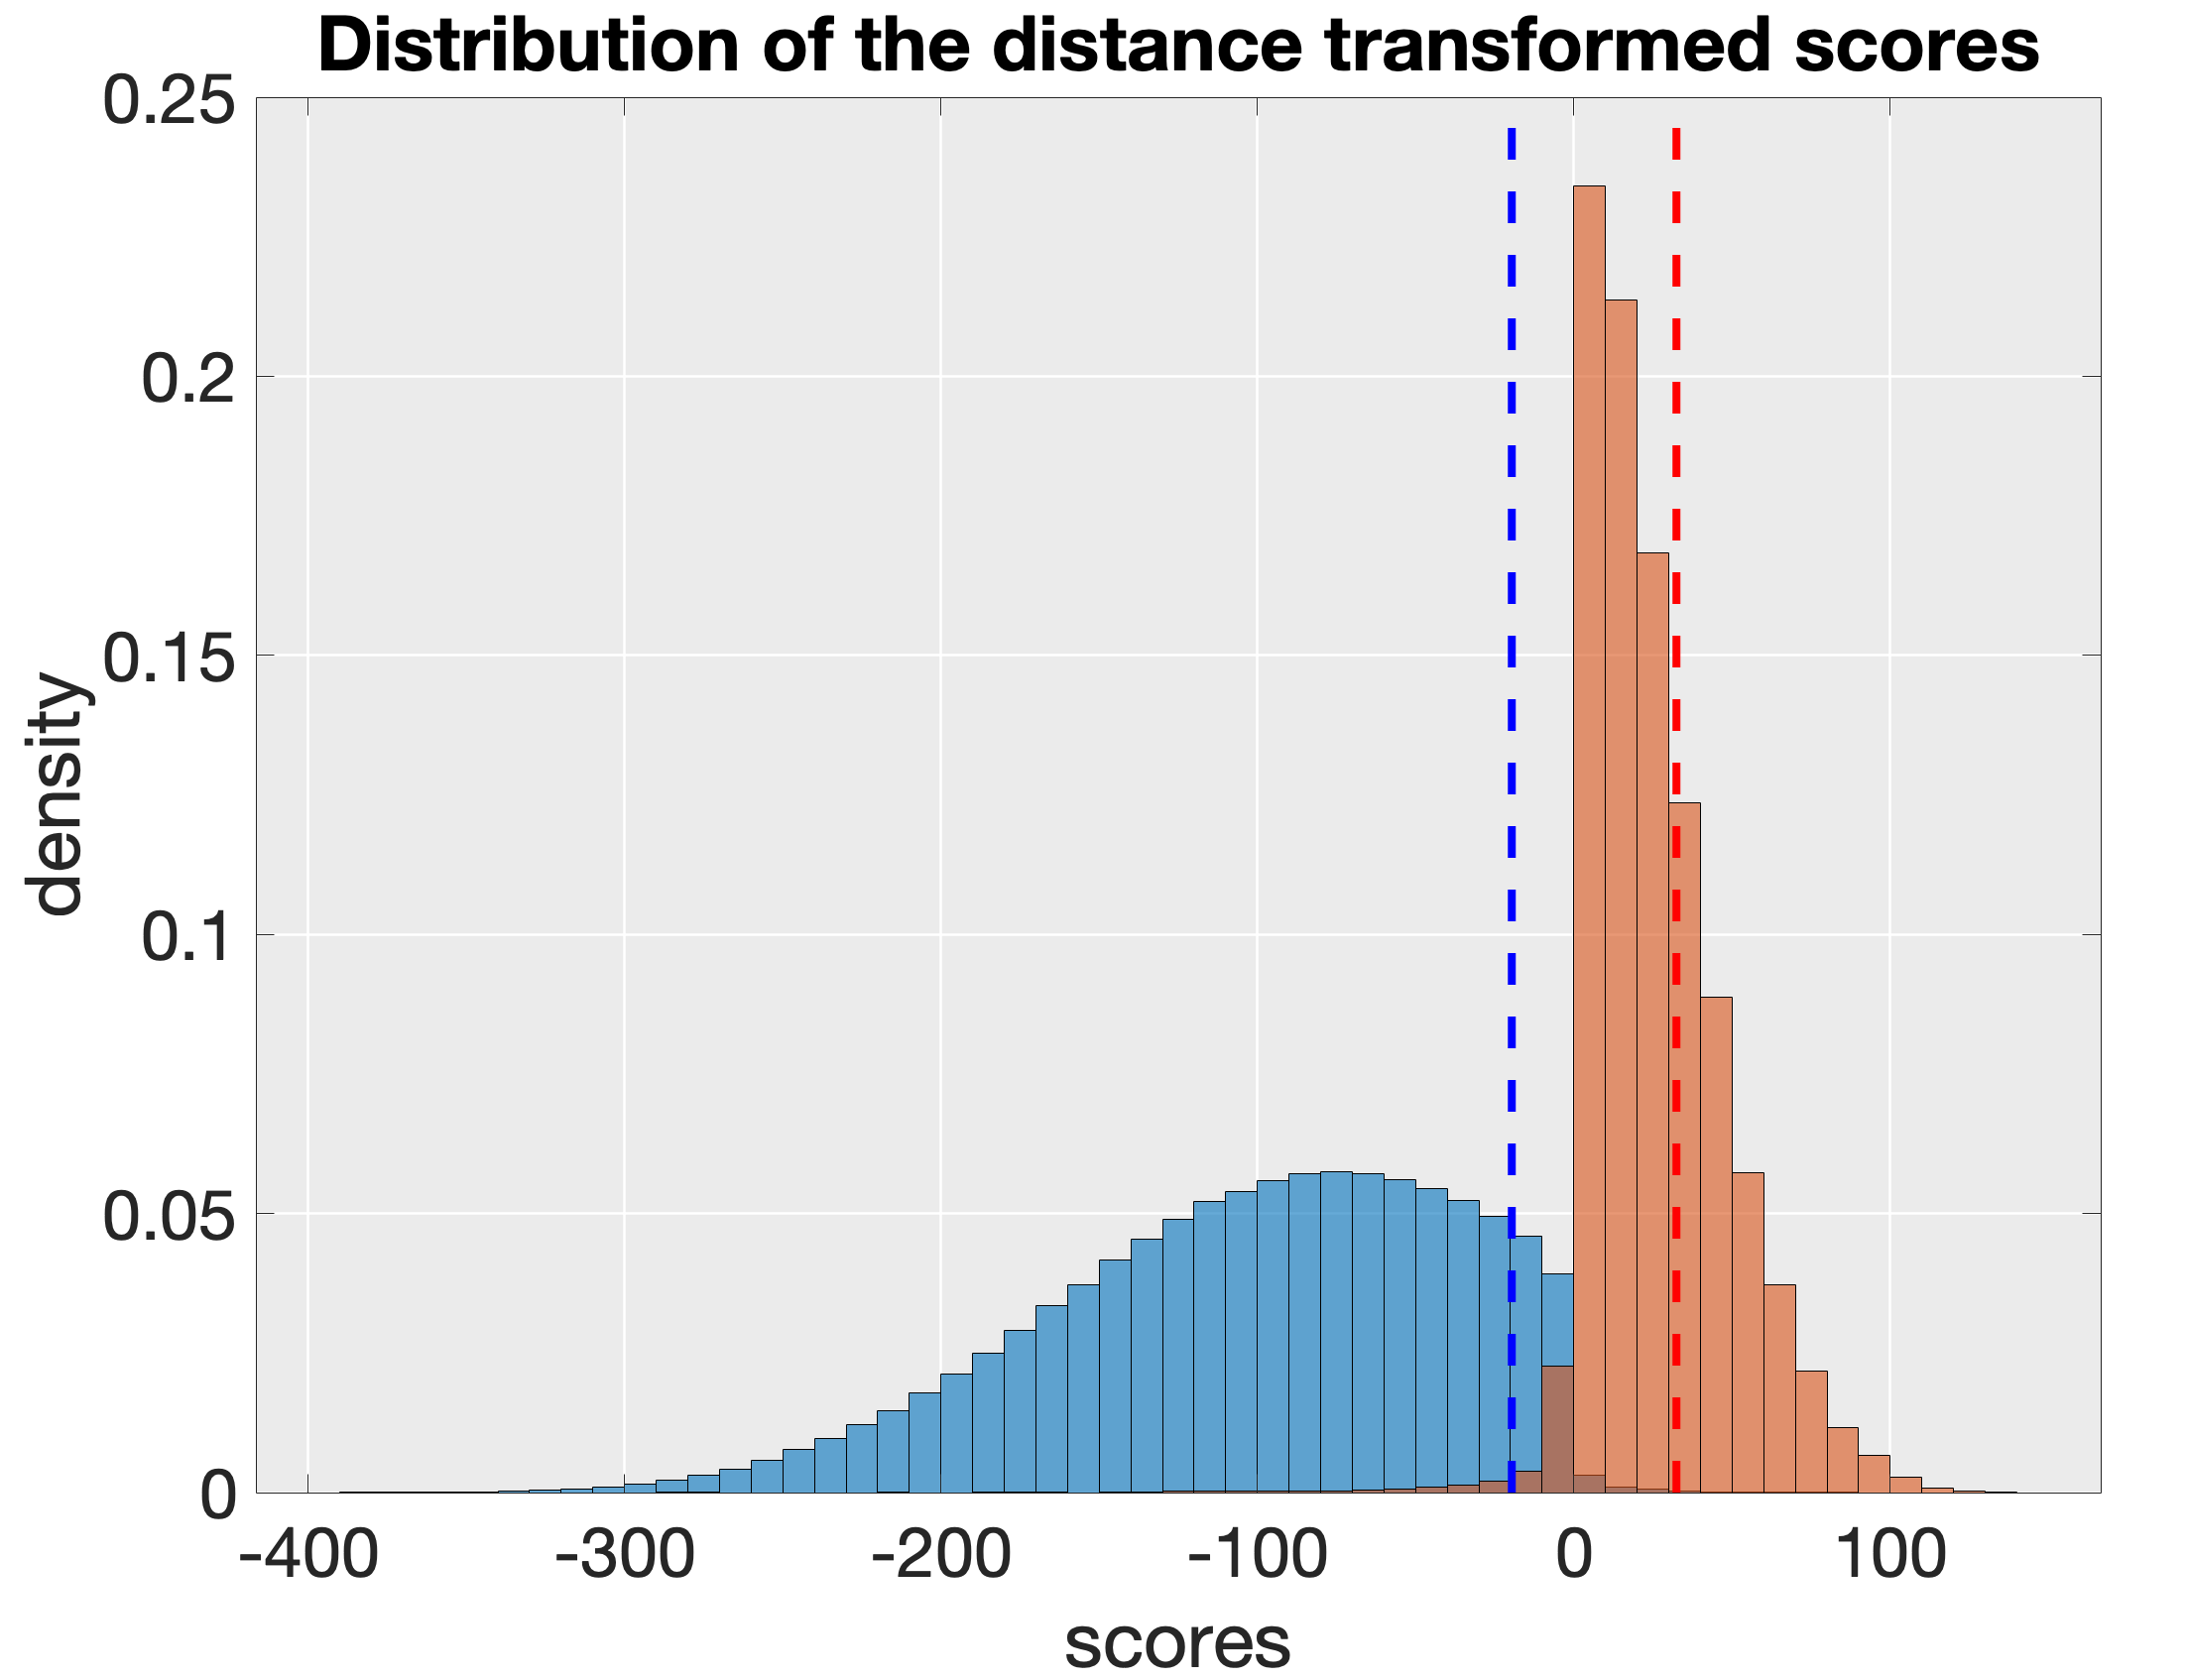
\includegraphics[width=0.3\textwidth]{../figures/learning/distscores.png}
	\label{scorehists}
\end{figure}


%\subsection{Tumor detection}
%\begin{figure}[h!]
%	\centering
%	\includegraphics[width=\textwidth]{tumorfwerimage.png}
%	\caption{Examples}
%	\label{fig:enter-label}
%\end{figure

%\subsection{}
\subsection{Illustrating the performance of conformal confidence sets}\label{SS:val}
Based on the results of the learning dataset we decided to combine the best of the approaches for the inner and outer sets respectively, taking $f_I$ to be the softmax transformation and $f_O$ to be the distance transformation of the predicted mask.

We divide the 1500 images at random into 500 for conformal calibration, and 1000 for validation. The resulting conformal confidence sets for this data are shown in the second row of Figure \ref{fig:polpys}. For comparison we have also shown the sets obtained based on the untransformed softmax scores in the top row. From this figure we see that the method, using the transformed scores, effectively delineates polyp regions. Inner sets are plotted in red and the outer sets are shown in blue. The ground truth mask for each polpys is shown in yellow and can be compared to the original images. In each of the examples considered the ground truth mask is bounded from within by the inner set and from without by the outer set. 

\begin{figure}
	\begin{subfigure}{0.19\textwidth}
		\centering
		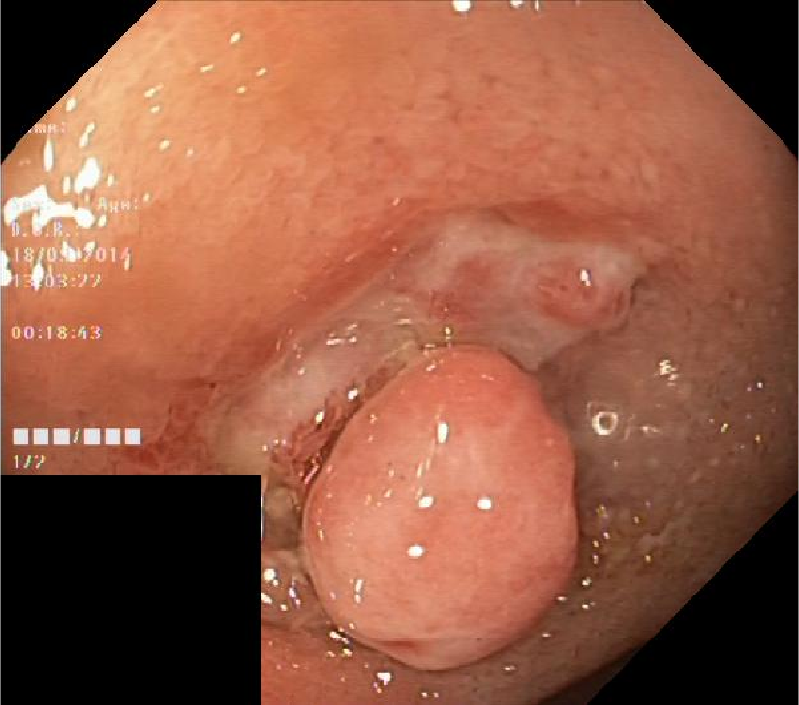
\includegraphics[width=\textwidth]{../figures/val_images/15.png}
		\label{fig:1}
	\end{subfigure}
	\begin{subfigure}{0.19\textwidth}
		\centering
		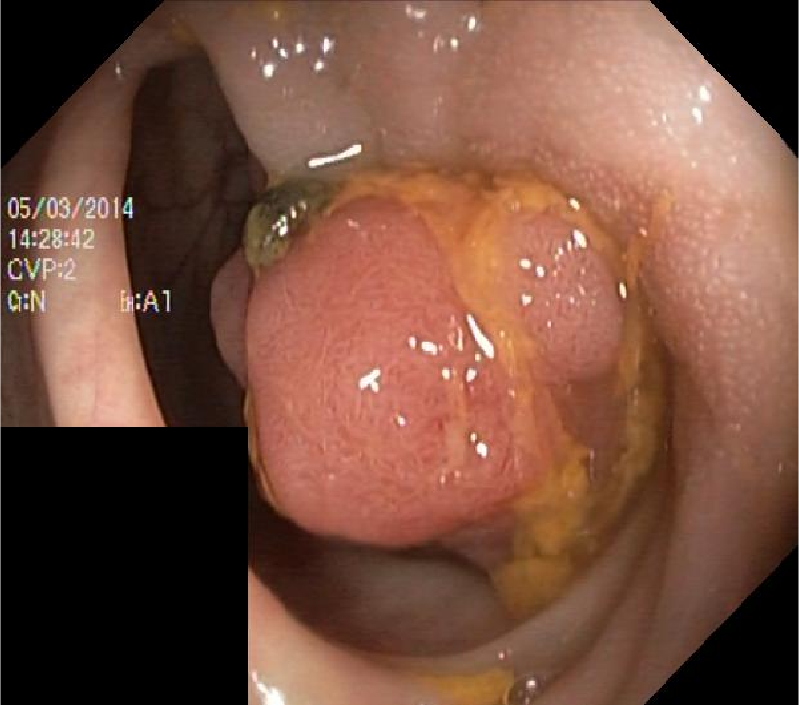
\includegraphics[width=\textwidth]{../figures/val_images/114.png}
		\label{fig:1}
	\end{subfigure}
	\begin{subfigure}{0.19\textwidth}
		\centering
		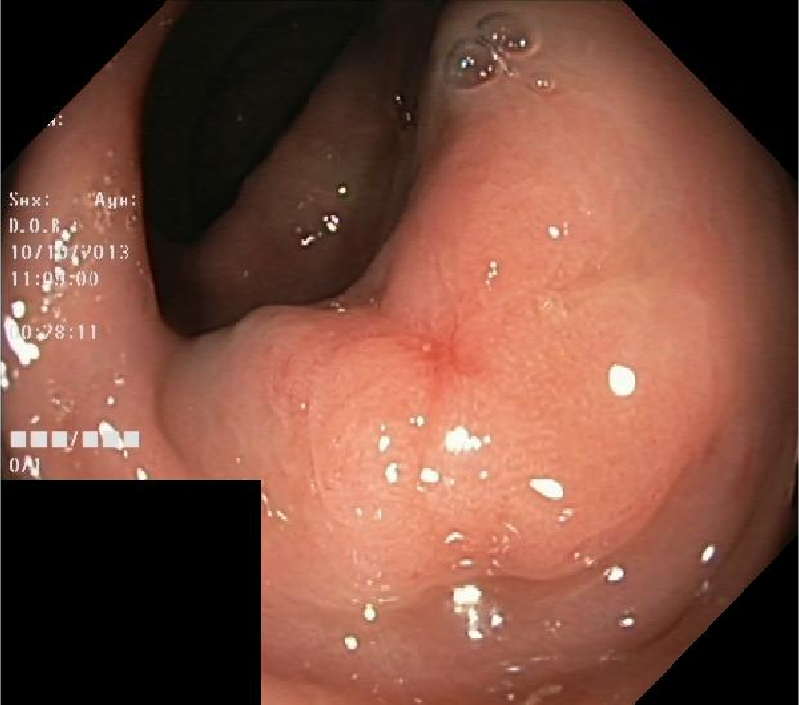
\includegraphics[width=\textwidth]{../figures/val_images/61.png}
		\label{fig:1}
	\end{subfigure}
	\begin{subfigure}{0.19\textwidth}
		\centering
		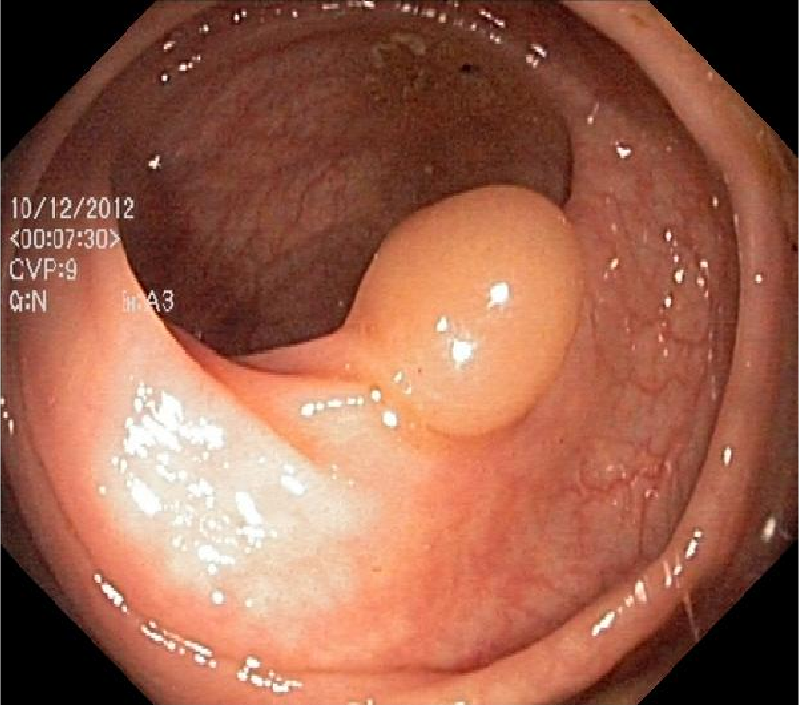
\includegraphics[width=\textwidth]{../figures/val_images/76.png}
		\label{fig:1}
	\end{subfigure}
	\begin{subfigure}{0.19\textwidth}
		\centering
		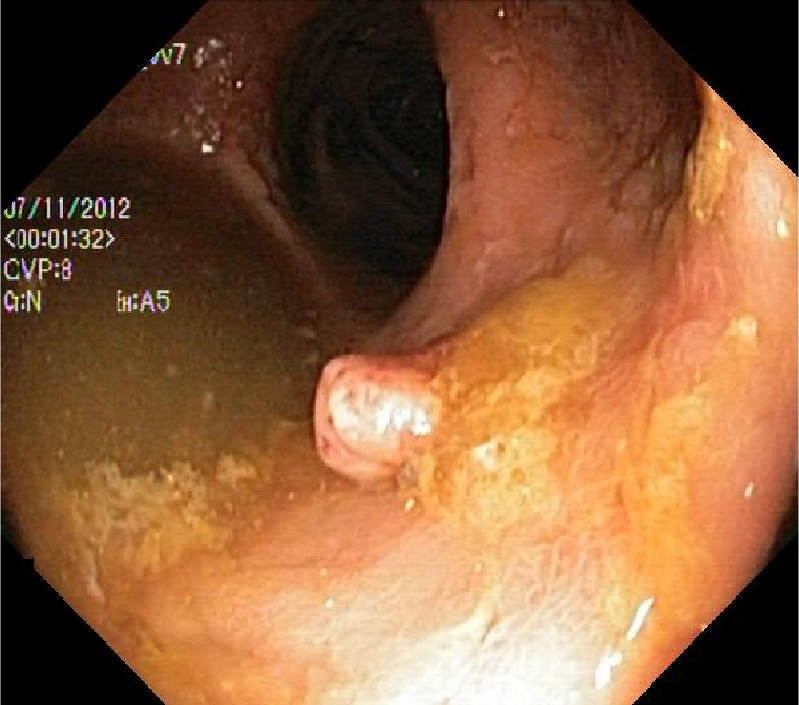
\includegraphics[width=\textwidth]{../figures/val_images/87.png}
		\label{fig:1}
	\end{subfigure}
		\vspace{-0.4cm}
	\\
		\begin{subfigure}{0.19\textwidth}
		\centering
		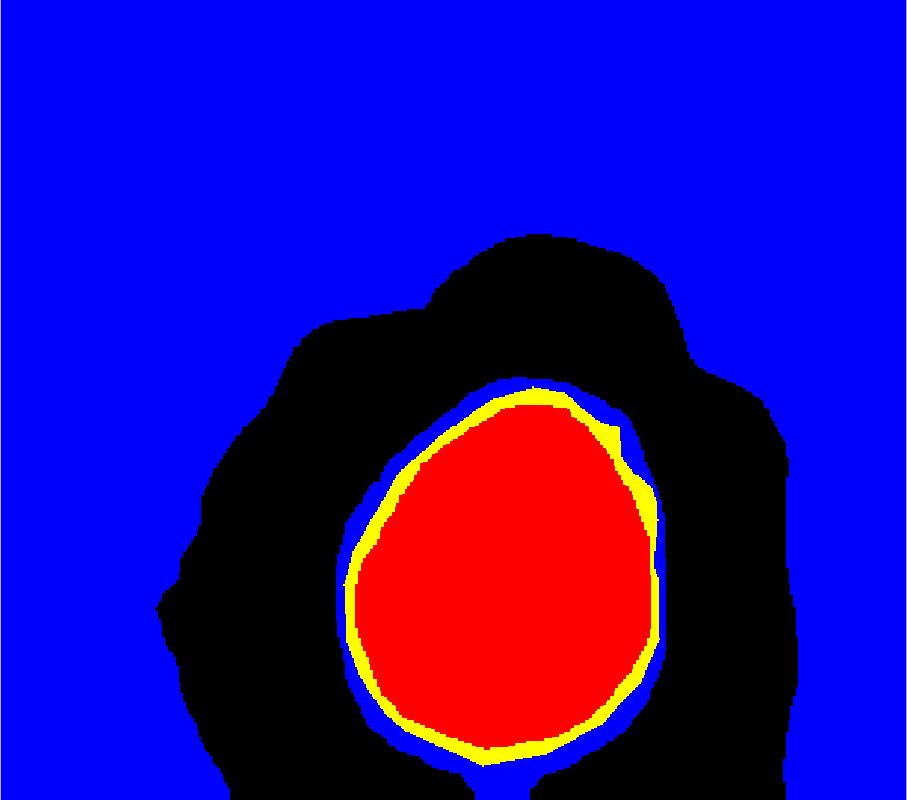
\includegraphics[width=\textwidth]{../figures/val_crs_90_orig/15.png}
		\label{fig:1}
	\end{subfigure}
	\begin{subfigure}{0.19\textwidth}
		\centering
		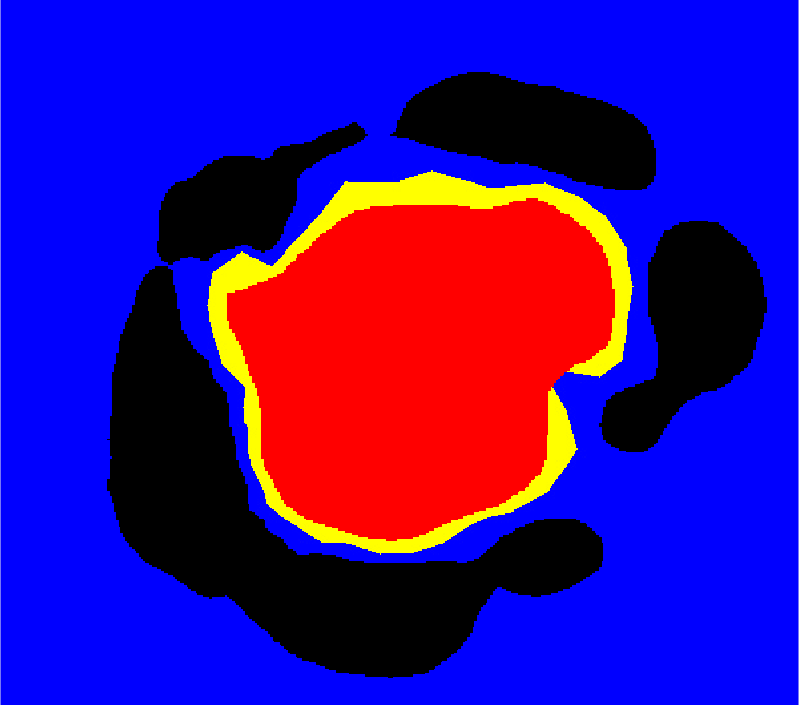
\includegraphics[width=\textwidth]{../figures/val_crs_90_orig/114.png}
		\label{fig:1}
	\end{subfigure}
	\begin{subfigure}{0.19\textwidth}
		\centering
		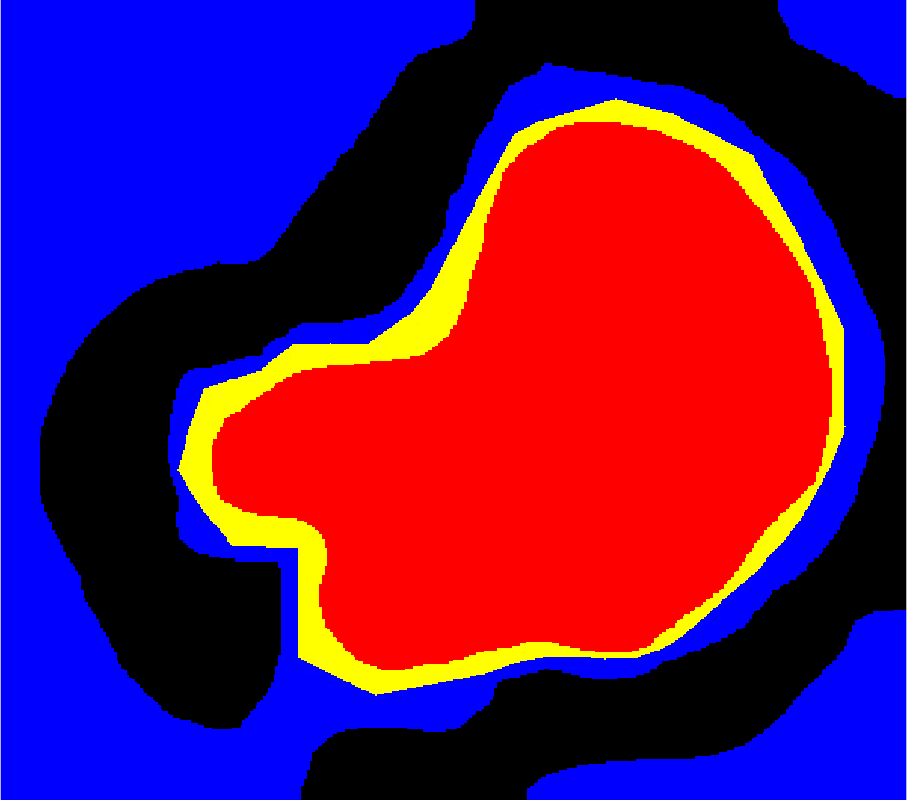
\includegraphics[width=\textwidth]{../figures/val_crs_90_orig/61.png}
		\label{fig:1}
	\end{subfigure}
	\begin{subfigure}{0.19\textwidth}
		\centering
		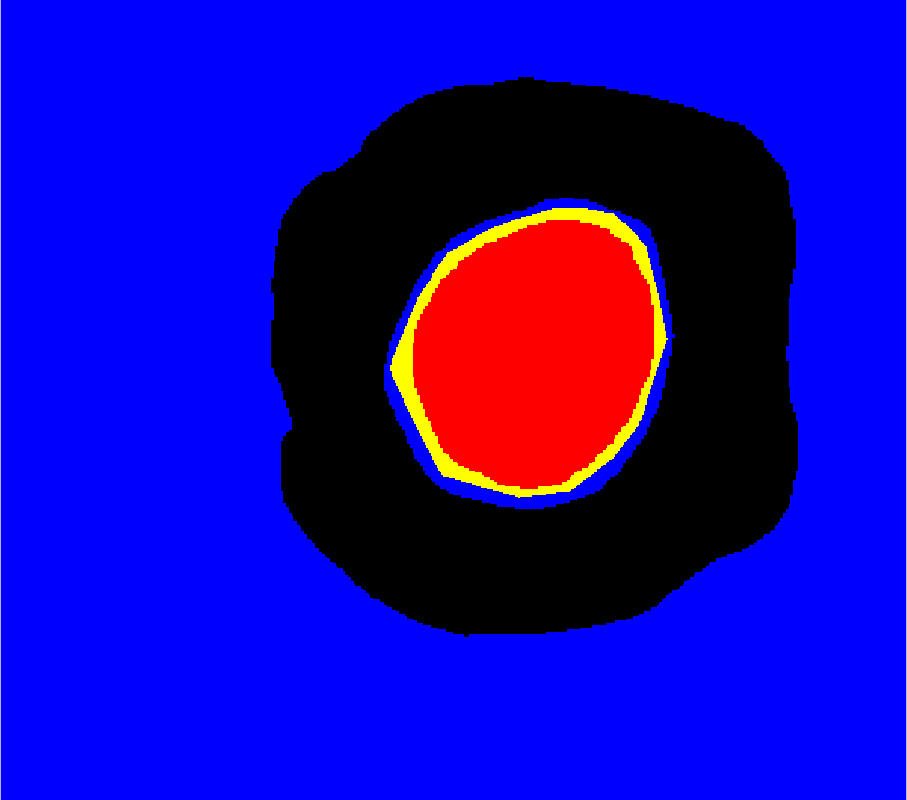
\includegraphics[width=\textwidth]{../figures/val_crs_90_orig/76.png}
		\label{fig:1}
	\end{subfigure}
	\begin{subfigure}{0.19\textwidth}
		\centering
		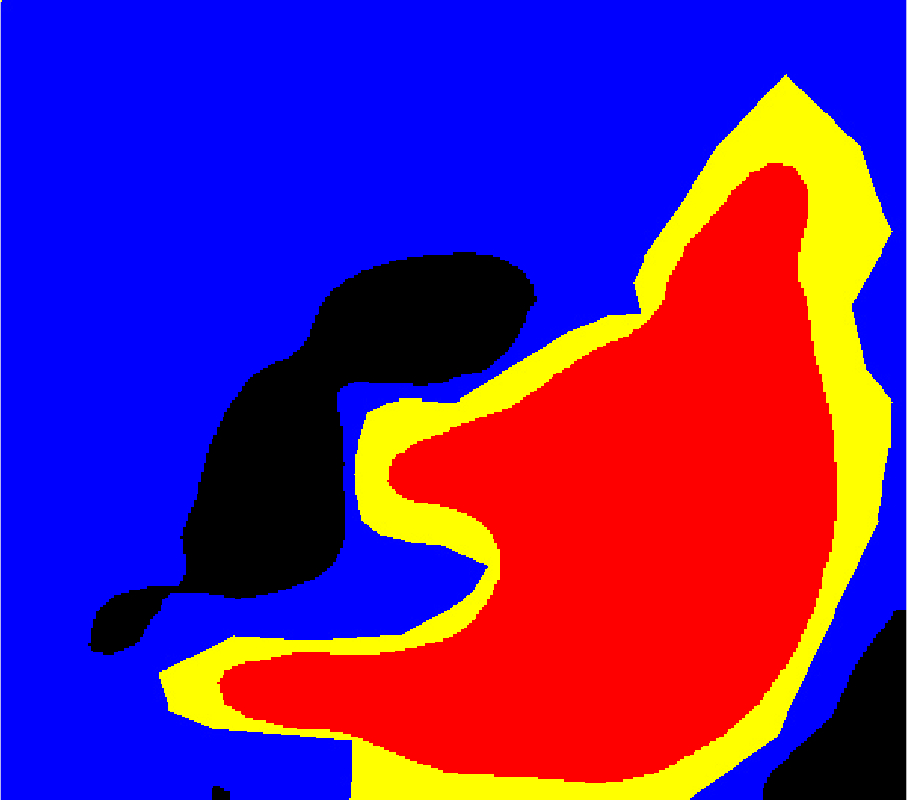
\includegraphics[width=\textwidth]{../figures/val_crs_90_orig/87.png}
		\label{fig:1}
	\end{subfigure}
	\vspace{-0.4cm}
	\\
	\begin{subfigure}{0.19\textwidth}
		\centering
		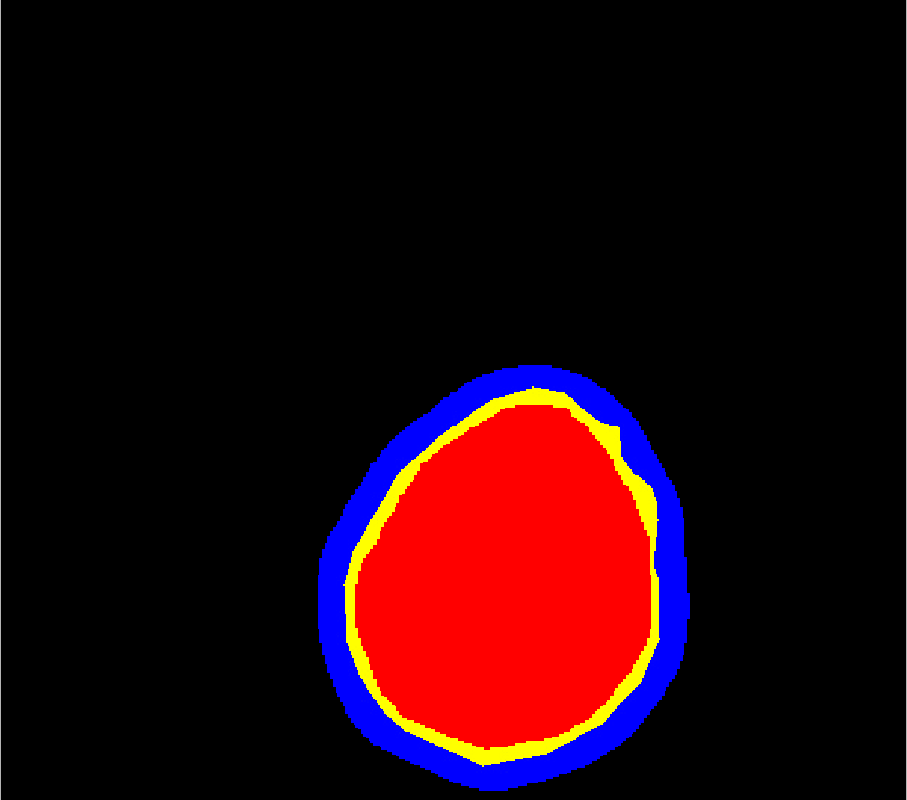
\includegraphics[width=\textwidth]{../figures/val_crs_90_distmix/15.png}
		\label{fig:1}
	\end{subfigure}
	\begin{subfigure}{0.19\textwidth}
		\centering
		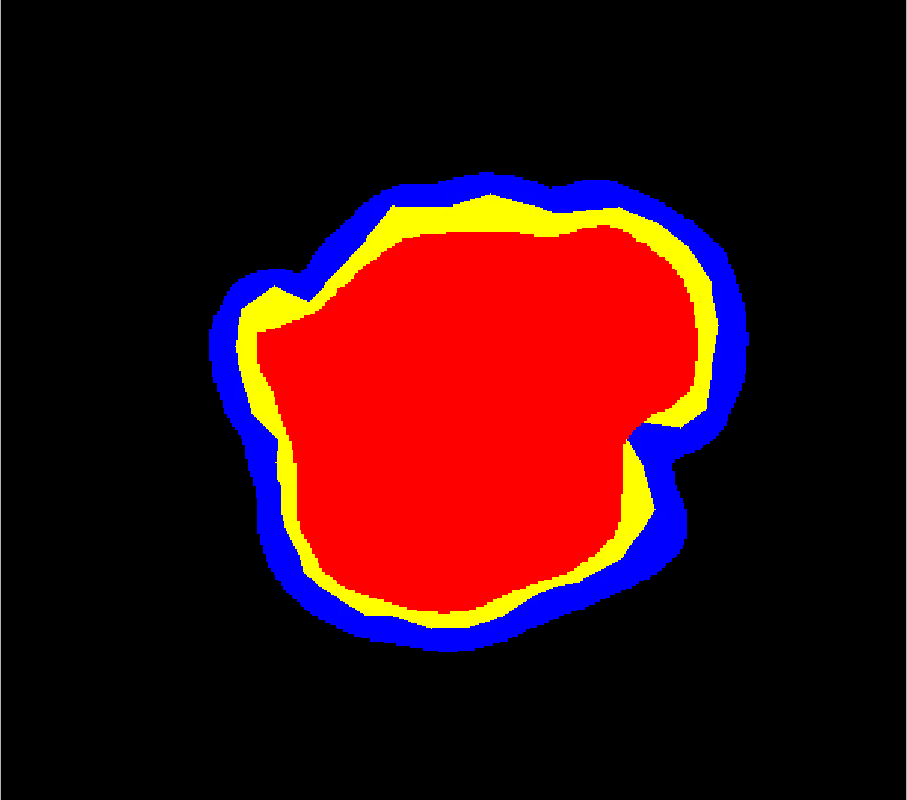
\includegraphics[width=\textwidth]{../figures/val_crs_90_distmix/114.png}
		\label{fig:1}
	\end{subfigure}
	\begin{subfigure}{0.19\textwidth}
		\centering
		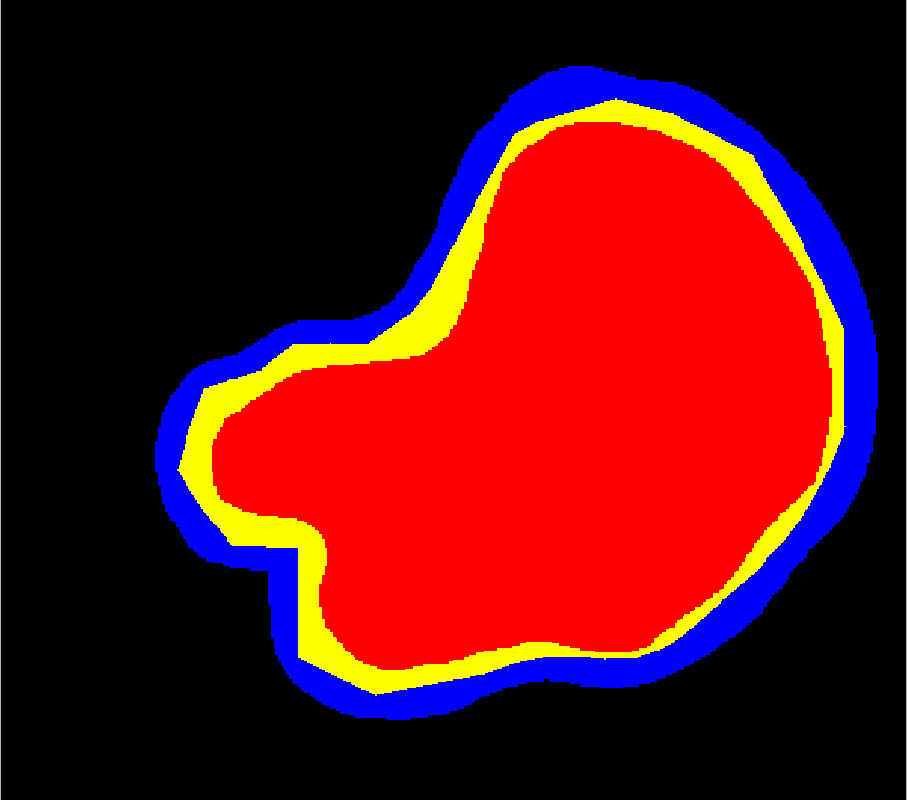
\includegraphics[width=\textwidth]{../figures/val_crs_90_distmix/61.png}
		\label{fig:1}
	\end{subfigure}
	\begin{subfigure}{0.19\textwidth}
		\centering
		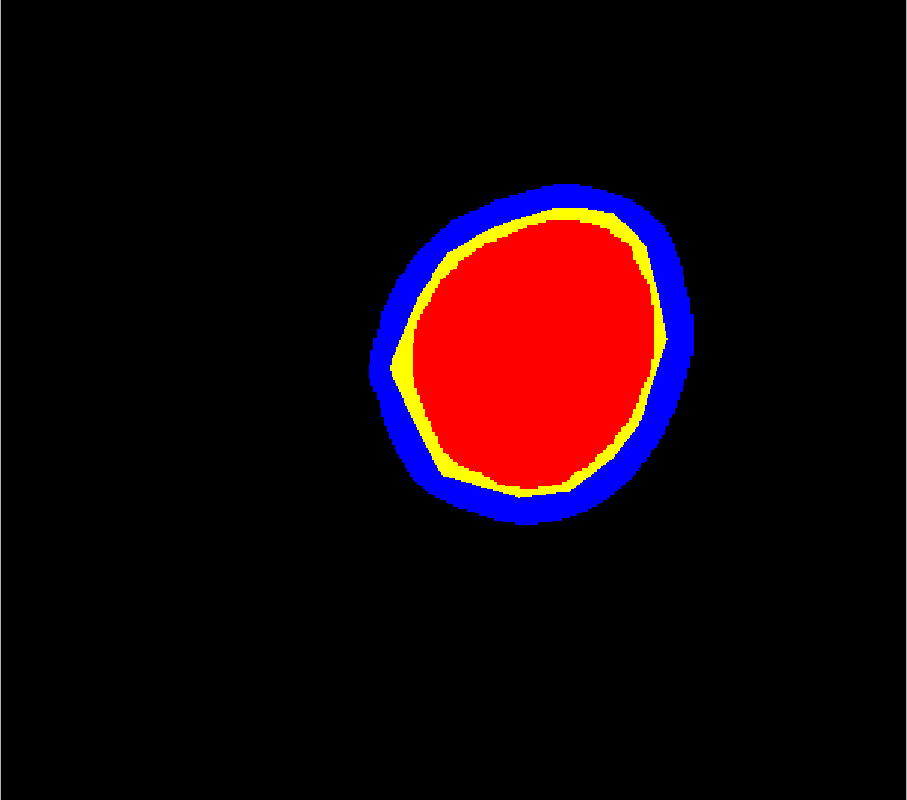
\includegraphics[width=\textwidth]{../figures/val_crs_90_distmix/76.png}
		\label{fig:1}
	\end{subfigure}
	\begin{subfigure}{0.19\textwidth}
		\centering
		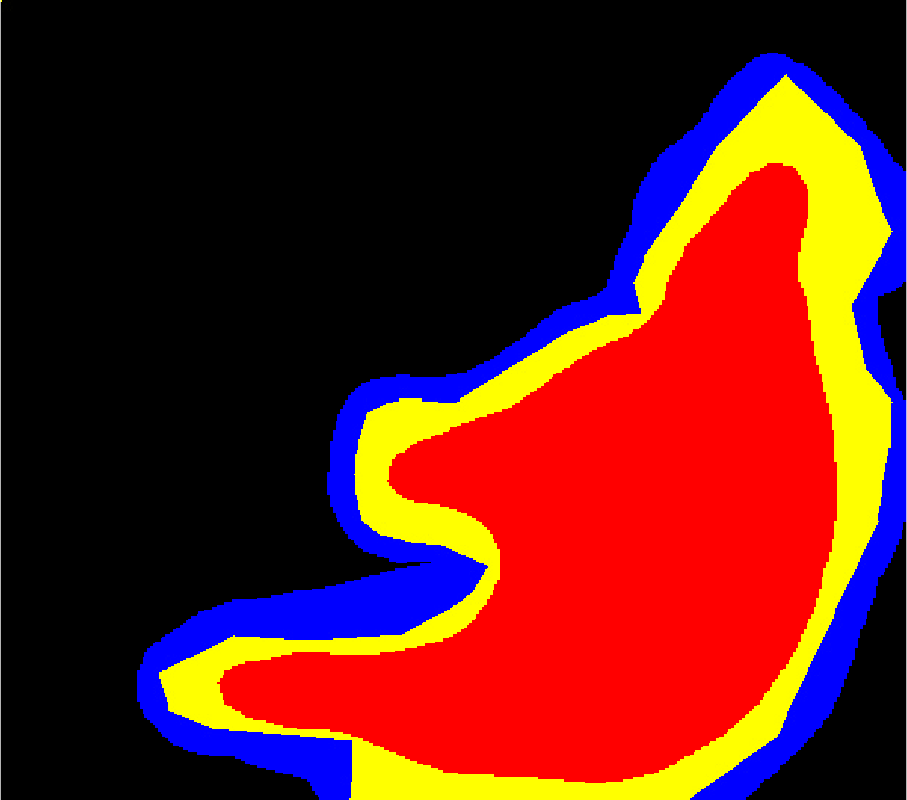
\includegraphics[width=\textwidth]{../figures/val_crs_90_distmix/87.png}
		\label{fig:1}
	\end{subfigure}
	\label{fig:grid}
	\caption{Conformal confidence sets for the polyps data. The bottom row shows the original endoscopic images with visible polyps. The top two rows present the conformal confidence sets, with the ground truth masks shown in yellow. The inner sets and outer sets are shown in red and blue respectively. The top row illustrates the sets which arise when using the original scores. Instead the middle show the resulting sets when $f_O$ is given by the distance transformation of the predicted polpys mask. The figure shows the benefit of transforming the score function and illustrates the method's effectiveness in accurately identifying polyp regions whilst providing informative spatial uncertainty bounds.}\label{fig:polpys}
\end{figure}


The inner sets are shown in red and represent regions where we can have high confidence of the presence of polyps. The outer sets are shown in blue and represent regions in which the polpys may be.

These results show that we can provide informative confidence bounds for the location of the polpys and allow us to use the PraNet segmentation model with uncertainty guarantees. They also illustrate the limitations of the model which is essential for applications. Larger uncertainty bounds may require specialist follow-up in order to be certain about the true extent of the observed tumor. Improved uncertainty quantification would require an improved segmentation model. 

More precise results can be obtained at the expense of probabilistic guarantees, see Figure XXX. A trade off must be made between precision and confidence and this can also be determined in advance based on the learning dataset. The approach of CITE controls the empirical false negative risk yielding additional precision but at the cost of coverage as shown in Figure XXX. 

\subsection{Measuring the coverge rate and efficiency}
In this section we run validations to evaluate the false coverage rate of our approach. To do so we take the set aside 1500 images and run 1000 validations, in each validation dividing the data into equally sized calibration and test sets of 750 images. In each division we calculate the conformal confidence sets using the above approaches and evaluate the coverage rate for $\alpha$ ranging from $0.05$ to $1$ on the test dataset. We average over all validations and present the results in Figure XXX. In this Figure we also compare to the coverage attained by using Bonferroni and Conformal Risk control \cite{}. We can see that Bonferroni whilst valid is conservative because it does not account for the dependence in the data. Instead conformal risk control can have highly inflated error rates - this is because it is designed to control the expected proportion of discoveries not cover the tumors. The results indicate the trade-off that must be made when choosing between the methodss, i.e. whilst risk control can provide meaningful inference CITE it comes with a cost in terms of under coverage. Instead, in this setting, conformal confidence sets provide informative segmentation bounds (as illustrated in Section \ref{SS:val}) and come with strong coverage guarantees.

\begin{figure}
	
	\caption{Left: . Right: False coverage rate of the outer and inner sets over the test set of 1000 images for $\alpha$ ranging from 0 to $0.2$.  }\label{fig:dist}
\end{figure}

\begin{figure}
	content...
	\caption{Measuring the efficiency of the bound. In this figure we plot }
\end{figure}

\subsection{Improving risk control using transformed scores}
Risk control can also benefit  
 
%\subsection{Application to Melanoma segmentation}

%\subsection{Melanoma Lesion Segmentation}

%\subsection{Melanoma Segmentation}
